\thispagestyle{empty}
\begin{center}
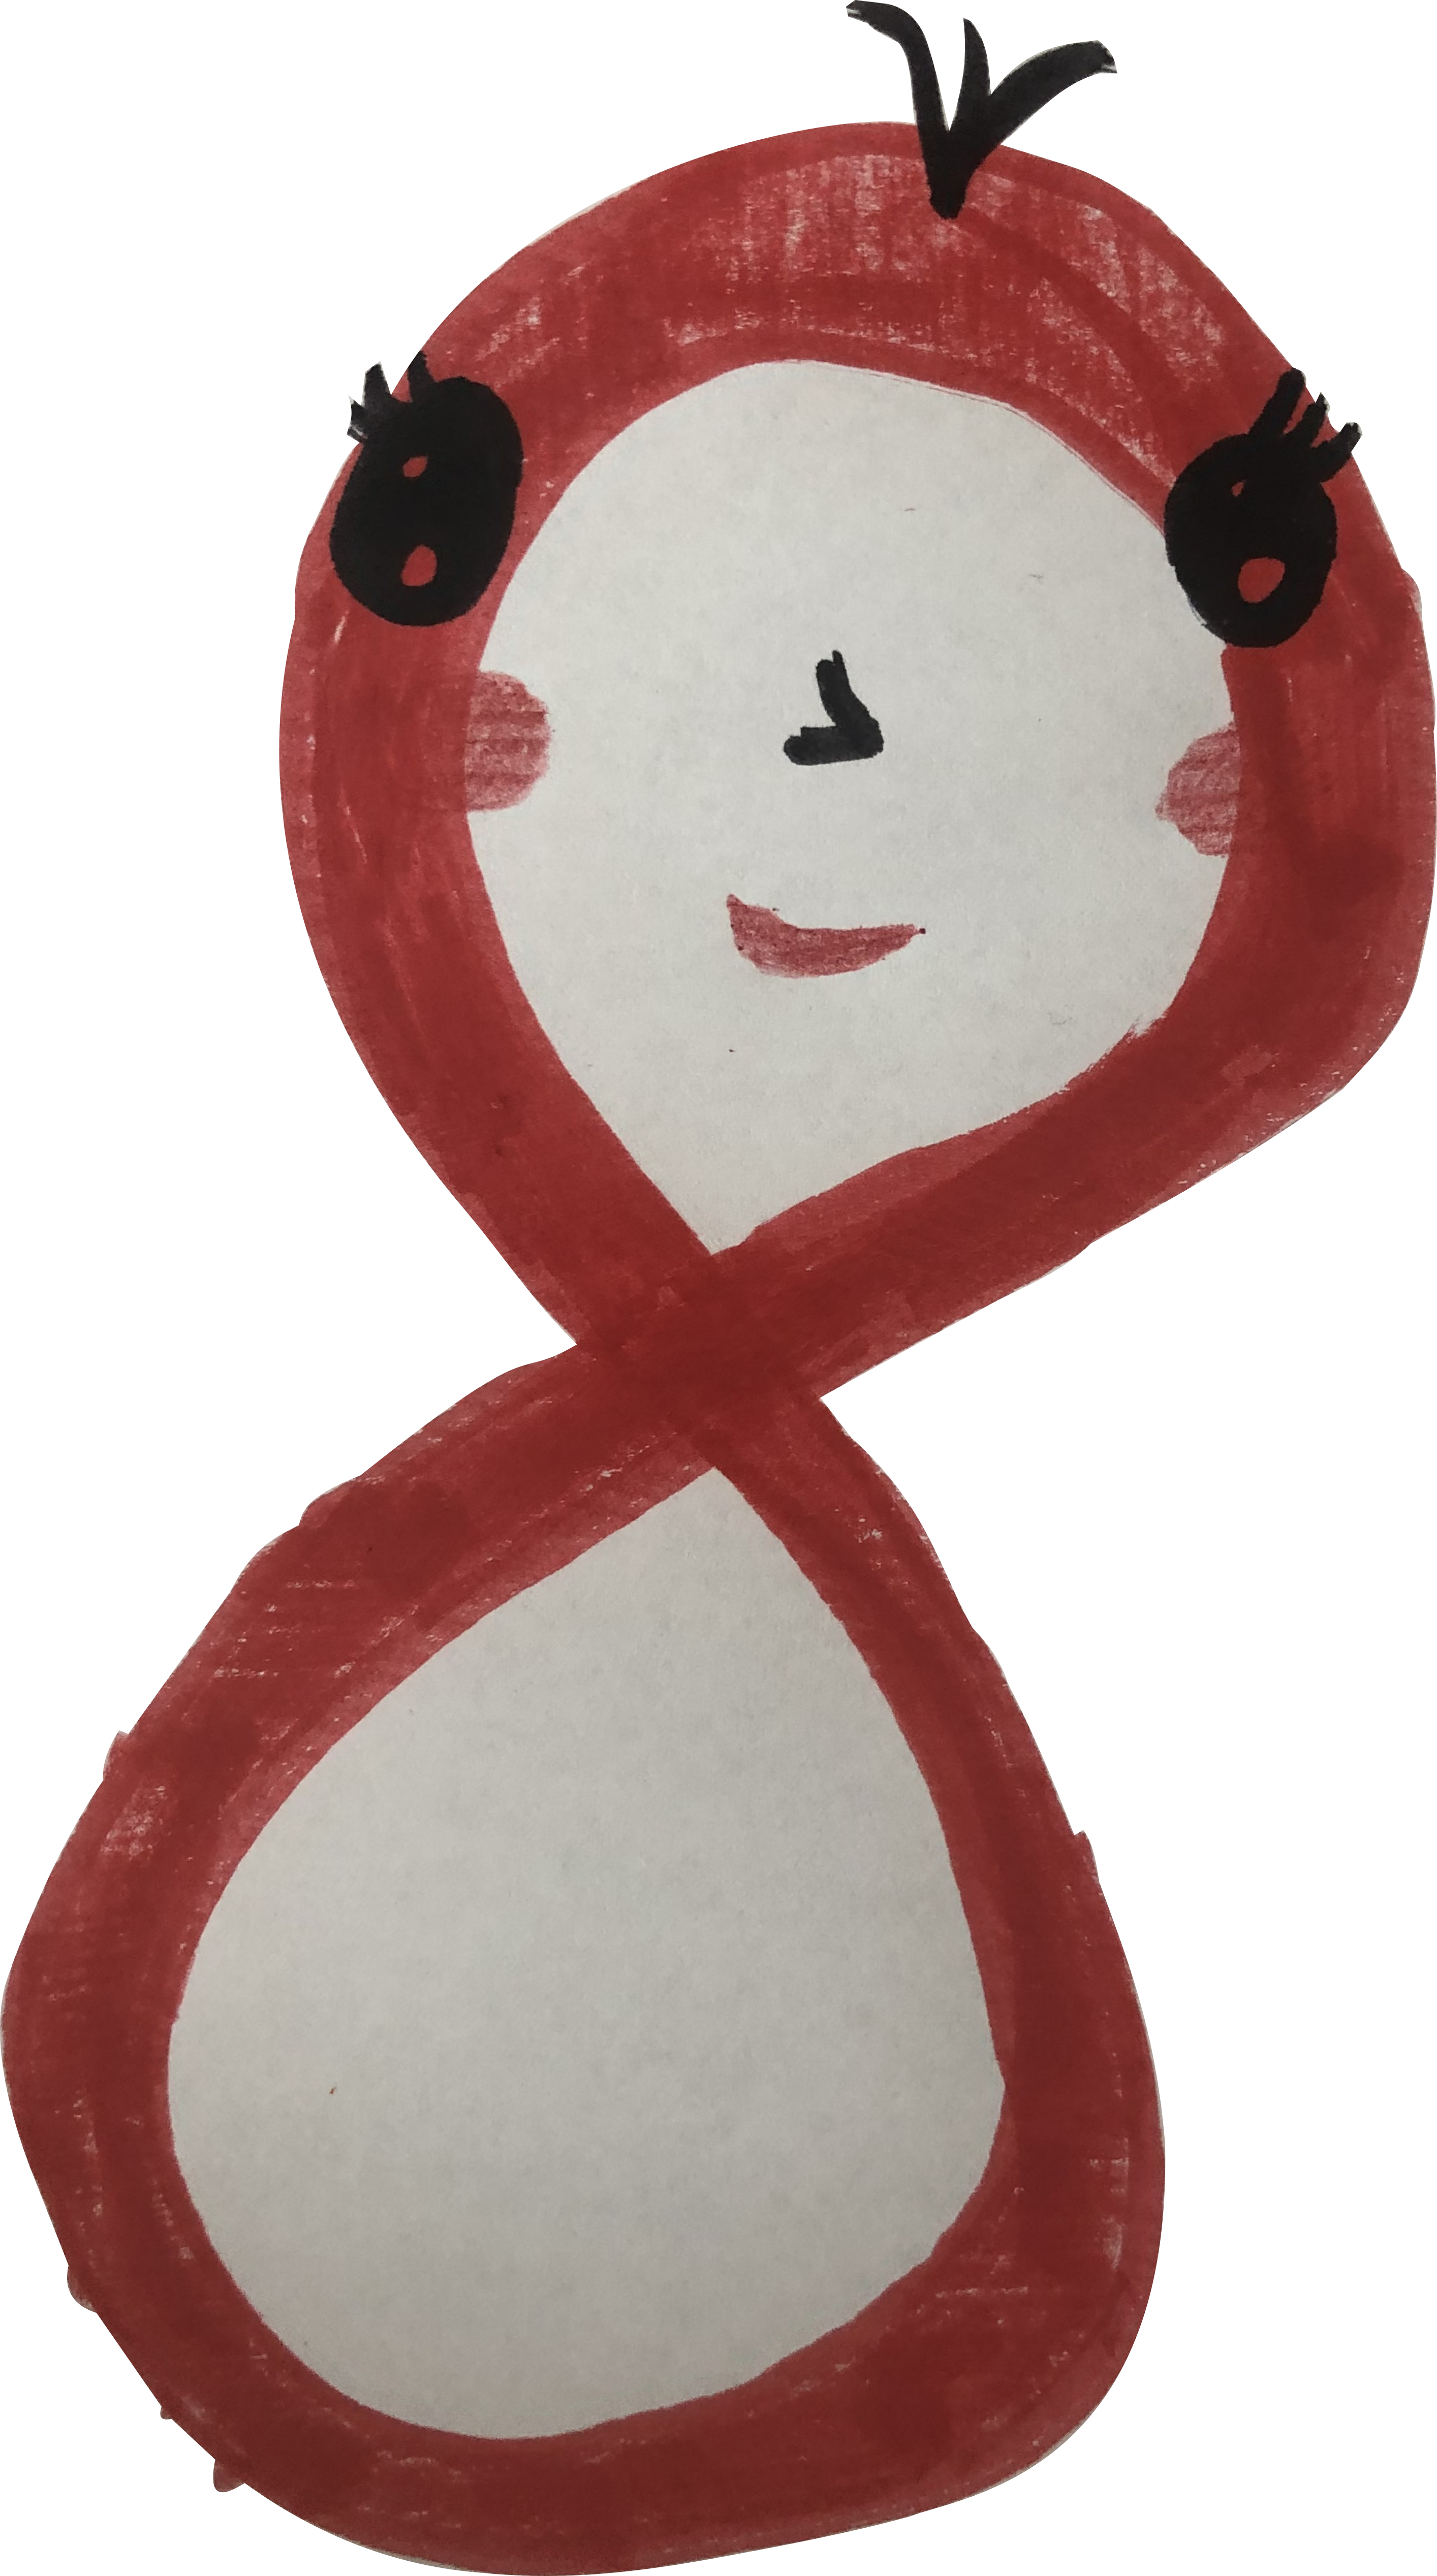
\includegraphics[height=.8\textheight]{./bilder/acht_1.png}
\end{center}
\vspace*{\fill}
%{\Huge\color{farbe}\hfill{\ttfamily{Fangen}}}
{\centering\fontsize{50}{48} \color{farbe}\sffamily{Das \textbf{X} ist los}\par}
\addcontentsline{toc}{chapter}{Das X ist los}
\newpage
%%%%%%%%%%%%%%%%%%%%%%%%%%%%%%%%%%%%%%%%%%%%%%%%%%%%%%%%%%%%%%%%%%%%%%%%%%%%%%%
\lettrine[lines=3, lhang=.2, loversize=.25, lraise=0.05, findent=0.1em,
nindent=0em]{W}{ieder} einmal wurde die \Circled{8} auf dem Schulhof der Zahelnschule gehänselt. \enquote{Brezel, Brezel} riefen die anderen Zahlenkinder. Die \Circled{1} hielt sich für die Königin aller Zahlen, weil sie vor allen anderen kommt. Die \Circled{7} dachte, dass alle ausser ihr dick sind und zwar vor allem die \Circled{8} und das sagte sie ihr auch immer wieder. Die \Circled{9} ist die grösste von allen und liess das alle spüren. Die \Circled{4} dagegen hatte sogar schon lackierte Fingernägel und nur Markenklamotten, dabei war sie noch nicht einmal zweistellig!

Nur die \Circled{8} hatte nichts, womit sie irgendjemanden beeindrucken konnte. Heute zum Beispiel war Mitbringtag in der Schule. Der war immer kurz nach den Ferien. Alle brachten was von zuhause mit, dass sie den anderen zeigen konnten. \Circled{8} hatte ihr Lieblingsplüschtier mitgebracht, ein zuckersüsses kleines \Circled{g}. Als sie aber gesehen hatte, was die anderen alle Tolles haben, hat sie sich gar nicht getraut, das \Circled{g} aus ihrer Tasche zu nehmen und behauptet, sie hätte das ganz vergessen.

Vermutlich hätte es aber sowieso niemand gemerkt. Die \Circled{3} hatte Gipfeli mitgebracht. Ihre Eltern führten eine Bäckerei. Warum hatte sie nicht so spannende Eltern? Die machten irgendwas Langweiliges im Büro. Die \Circled{1} hat sich mit lauten Seufzen und dem Ruf \enquote{Meine Lebensretterin, ich verhungere.} gleich zwei Gipfeli genommen. Das dafür \Circled{8} keines ab bekam kommentierte sie mit \enquote{Ich wollte sowieso keines.} Stimmte aber gar nicht, natürlich hätte sie sogar liebend gerne eines gegessen, selbst wenn sie die sonst nie lecker gefunden hätte.

Solange die anderen wie sie fand übertrieben laut kauten, kramte \Circled{8} in ihrem Etui, um so zu tun, als sei sie schwer beschäftigt. Die Schulklingel erlöste sie aus der ewig dauernden blöden Situation. Frau Zahl kam hektisch zur Tür hereingestürmt, sie kam immer genau zum Klingeln. Wie macht sie das bloss, fragte sich \Circled{8}, wartet sie vor der Tür oder stellt sie sich die Uhr und hat vorher ausgemessen, wie lange sie braucht?

Was allerdings anders war als sonst: Diesmal kam noch jemand hinter Frau zahl durch die Tür geschlüpft. Ein Kind, aber es sah sonderbar anders aus als die anderen hier in der Klasse.

\enquote{Ruhe bitte, alle auf ihre Plätze!}, die Aufforderung gehörte zu jedem Tag dazu. \enquote{Liebe Klasse}, fuhr Frau Zahl fort, nachdem das letzte Getuschel durch strenge Blicke beendet worden war, \enquote{Ich möchte euch eure neue Mitschülerin vorstellen, das ist \Circled{13}. Stell dich doch am besten selber vor.}

Die \Circled{13} war gar nicht schüchtern. Alle hatten das Gefühl, dass sie nur sie ansieht.

\enquote{Ich bin \Circled{13}. Ich mag Abenteuer, Rechnen und Netflix.}

Alle kicherten und Frau Zahl nickte zustimmend, als hätte \Circled{13} gerade die richtigen Antworten in einem mündlichen Test gegeben.

\enquote{Prima. Du kannst dich neben \Circled{8} setzen.} Wieder kichern alle, diesmal weiss aber niemand warum.

Was Frau Zahl als nächstes alles erklärte, bekam \Circled{8} nicht mit. Sie musste die ganze Zeit aus den Augenwinkeln zu \Circled{13} schielen, hoffentlich merkte die das nicht. Aha, als es im Klassenzimmer anfängt zu rascheln, weil alle ihre Hefte und Stifte aus dem Pult holen, merkt auch \Circled{8}, was sie machen soll. Aufschreiben, was sie in den Ferien erlebt hat. \Circled{13} bleibt ganz lässig. Nach einer Ewigkeit nimmt sie ihren Bleistift, fängt aber nicht an zu schreiben, sondern spitzt den Stift erst einmal ganz in Ruhe. \Circled{8} ist neidisch, so cool wäre sie auch gerne mal. Dann fängt \Circled{13} aber doch an zu schreiben:

\enquote{In diesem Sommer bin ich verreist und doch nicht verreist. Ferien mit Baden und Hotel haben wir jedenfalls nicht gemacht, wir sind umgezogen. Das Einpacken und Auspacken hat keine Zeit übriggelassen. Alle meine Freundinnen wohnen noch da, wo ich früher gewohnt habe. Hier kenne ich niemanden, nicht einmal die Lehrerin, deren Namen ich schon wieder vergessen habe. Meine Lehrerin früher war ein Lehrer und hiess Herr Nummero. Der war immer sehr nett und hat viele Witze gemacht.}

Den letzten Satz will \Circled{13} durchkritzeln, aber man kann ihn immer noch lesen. \Circled{8} kramt wieder in ihrem Etui und reicht ihr ihren Lieblingsradiergummi, der aussieht wie eine Erdnuss. \Circled{13} nimmt ihn und lächelt \Circled{8} zu.

Noch während die letzten Kinder geschrieben haben, öffnete sich die Tür zum Klassenzimmer und der merkwürdigerweise immer fröhliche Direktor Herr Prim kam herein.

\enquote{Kinder, Kinder, Kinder, allerwerteste Kollegin Zahl, ich will gar nicht lange stören. Ich habe eine gute und eine schlechte Nachricht. Die schlechte zuerst: Morgen fällt der Unterricht leider aus.}

Na soo schlecht klang das jetzt für keines der Kinder, bei Frau Zahl war sich \Circled{8} nicht so sicher.

\enquote{Und die Gute: dafür gehen wir morgen in den Zoo, den haben wir sogar für uns alleine, denn eigentlich ist er ja gerade geschlossen.} Und lachend fügte er hinzu:

\enquote{Das habt ihr nur eurem super Direktor zu verdanken und ein ganz kleines bisschen seiner Schwester, die dort arbeitet. Wir treffen uns morgen zu Schulbeginn auf dem Schulhof und bis dahin tschüüüüss.} Ohne eine Reaktion der Klasse abzuwarten, war er schon wieder verschwunden.

Alle jubelten. Frau Zahl rief zwar etwas, aber niemand hörte zu. Endlich schaffte sie es doch, die Aufmerksamkeit wieder auf sich zu lenken. Ihre wirklich laute Stimme war da eine grosse Hilfe.

\enquote{Ich merke, heute wird es nichts mehr mit normalem Unterricht.}, erklärt sie und es klang wie eine Niederlage, die tapfer akzeptiert wird. \enquote{Dafür gibt es aber eine Hausaufgabe. Zusammen mit euren Sitznachbarn sucht ihr euch ein Tier aus dem Zoo aus und bereitet einen kurzen Vortrag für morgen vor.}

\Circled{8} und \Circled{13} sahen sich an. \enquote{Ein \Circled{G}} schlug \Circled{8} vor. \enquote{Oder lieber ein \Circled{A}?}, fragte \Circled{13}. Zum Schluss einigen sich beide auf ein \Circled{S} und darauf, dass \Circled{13} nach der Schule mit zu \Circled{8} kommt.

Am nächsten Tag hatten \Circled{8} und \Circled{13} nichts vorbereitet. Natürlich hatten sie den Nachmittag zusammen verbracht, aber bevor sie anfangen konnten, musste \Circled{8} \Circled{13} ihr Lieblingskartenspiel \textit{Drecksau} zeigen, verlor aber gleich die erste Runde. Eine Revanche führte zur nächsten bis es Abend wurde und \Circled{13} gehen musste.

Und jetzt standen sie hier. \Circled{4} und \Circled{9} redeten gerade über \Circled{A}s, die von Baum zu Baum springen, sich von Blättern ernähren und sich als solche tarnen, weswegen sie sich häufig gegenseitig in den Fuss beissen. Dagegen haben sich auf ihren Füssen kleine Schilde gebildet, weswegen die Füsse aussehen wir fünf kleine grüne Schildkröten.

\Circled{3} und \Circled{1} stellten \Circled{E}s vor, sagten aber nur, dass ihr Hauptmerkmal der lange Rüssel sein, als ob den jemand übersehen konnte.

\Circled{8} und \Circled{13} wurden immer nervöser. Gleich waren sie beim Gehege der \Circled{S}, also sie beide dran. Sie versuchten sich hinter dem Gehege der \Circled{E}s zu verstecken, um schnell mit dem Telefon im Internet nach ein paar Informationen zu suchen.

Doch plötzlich hörten sie ein lautes Krachen, ganz so, als wäre ein grosser Ast abgebrochen und dann ein Fauchen. Das musste aus der Richtung kommen, wo die \Circled{X} waren, dem Highlight des Zoos. Man bekam schon Gänsehaut, wenn man sie hinter der doppelten Absperrung sah.

Und tatsächlich, da kam ein riesiger \Circled{X} auf sie zu! Aber nicht im Gehege hinter vielen Zäunen, sondern hier, auf dem Weg für die Besucher, direkt vor ihnen. Die Sonne glitzerte in den Augen des \Circled{X}, aber es hatte \Circled{8} und \Circled{13} noch nicht bemerkt. Es lief auf der gegenüberliegenden Seite um das \Circled{A}-Gehege, genau in Richtung der nichtsahnenden Klasse.

\enquote{Was machen wir jetzt?} Beide trauten sich nicht zu bewegen.

\enquote{Ablenken, wir müssen es von den anderen verscheuchen.}, antwortete \Circled{8}, wusste aber auch nicht, wie.

\enquote{Bist Du verrückt? Wir müssen fliehen, abhauen, weg von hier!}.

\Circled{8} dachte zwar für einen ganz kurzen Augenblick an die vielen Male, die sie gehänselt worden war, sagte aber selbstverständlich:

\enquote{Das kommt gar nicht in Frage! Dort drüben ist das \Circled{X}-Gehege. Die Tür steht offen, ich schreie jetzt und flüchte dort hinein. Du gehst hier aussen herum und warnst die Klasse!}

Und ohne eine Antwort abzuwarten, schrie sie auch schon \enquote{\textit{Ahhhhhhhh}} und rannte los. Das \Circled{X} riss den riesigen Kopf herum, bleckte seine zwei Reihen messerscharfer Zähne und fixierte seine Beute. Nach all den Jahren im Käfig erwachte sofort das Raubtier, der Jäger in ihm wieder. Es senkte den Kopf, straffte so viele Muskeln wie ein Auto wiegt und sprang los. Damit war aber plötzlich der Weg für \Circled{13} abgeschnitten. Sie musste hinter \Circled{8} her.

Das merkte auch das \Circled{X}. Es schien zu wissen, was \Circled{13} vor hatte. \Circled{8} war bereits am Gehege angekommen. Gerade noch im letzten Augenblick bemerkte sie \Circled{13}, fast hätte sie schon die Tür zugeschlagen. Das \Circled{X} war jetzt in vollem Sprint. Seine Krallen schlugen laut auf den Boden, das Maul weit aufgerissen. Aber \Circled{13} schaffte es ins Gehege. Im allerletzten Moment schlug \Circled{8} die Tür zu. Aber die ging nicht mehr zu. Eine Tatze des \Circled{X} war schneller gewesen. Sie erwischte \Circled{8} am Arm. Die Tatze blockierte die Tür. \Circled{X} fauchte und brüllte und bis wild um sich. Ein kräftiger Tritt von \Circled{13} gegen die Tatze rettete beide. Krachend viel die Tür ins Schloss, sie waren sicher.

\Circled{8} blutete stark. Während das \Circled{X} tobend das Gehege umrundete, in dem es selber sonst steckte, riss \Circled{13} einen Ärmel ihrer Jacke ab und verband damit die Wunde. Beide waren bleich und zitterten. Dann folgte ein dumpfer Knall.

Das \Circled{X}, die \Circled{8} und die \Circled{13} sahen sich gleichermassen verwirrt um. Das \Circled{X} allerdings nicht lange. Es drehte sich noch zwei Mal um sich selbst und sank dann zusammen.

\enquote{Ist es tot?} \Circled{13} konnte auf die Frage nur mit den Schultern zucken. Jemand, der offensichtlich beim Zoo arbeitet, kam vorsichtig näher und vergewisserte sich, dass das \Circled{X} auch wirklich liegt. Mit dem Blick auf \Circled{8} rief er laut:

\enquote{Schnell, wir brauchen einen Arzt!} und dann mit Blick auf die beiden im Käfig:

\enquote{Ich habe das \Circled{X} nur betäubt und hole euch gleich da raus.}

Und noch während er versuchte, aus dem grossen Schlüsselbund den richtigen für das Gehege auszusuchen, kamen die anderen Kinder der Klasse angerannten, stoppten aber mit grossem Abstand zu dem \Circled{X}.
  
Während der Zoomitarbeiter die beiden befreite, klatschten die anderen. Eine Tierärztin kümmerte sich um das betäubte \Circled{X} und zusammen mit zwei anderen Mitarbeiterinnen zogen sie es zurück in den Käfig. 

\enquote{Das habt ihr prima gemacht}, sagte die Ärztin. \enquote{Ich bin so froh, dass niemandem etwas passiert ist!}

\enquote{Was passiert jetzt mit dem \Circled{X}}, fragte \Circled{13}. 

\enquote{Ess wird in zwei Stunden wieder aufwachen, wird die nächsten tage aber noch sehr durcheinander sein und braucht dann etwas Hilfe. Vor allem muss jemand aufpassen, dass es nicht wieder zusammen bricht, das passiert manchmal. Aber Moment, wollt ihr beiden das nicht übernehmen? Kommt einfach nach der Schule hier vorbei, dann könnt ihr mich ablösen und ich habe Zeit, zu den anderen Tieren zu sehen.} 

Und ohne eine Antwort abzuwarten, drehte sich die Ärztin zu iherer Mitarbeiterin um und beauftragte sie, zwei Zoomitarbeiterinnen-Ausweise zu organisieren. Aber dür die beiden Zahlenkinder war das auch keine Frage. Natürlich wollten sie! Aber erst musste \Circled{8} noch ins Krankenhaus, die Wunde richtig versorgen lassen. Aber auch das war eigentlich ein riesiger Spass. Erstens durfte \enquote{13} auch mit und zweitens fuhren sie mit Blaulicht durch die Stadt, extra wegen ihr, auch wenn der Rettungsarzt meinte, es sei wirklich gar nicht schlimm und es hätte nicht einmal einen Unterschied gemacht, zu Fuss zu laufen, aber als er die Geschichte der beiden gehört hatte, war so eine kleine Belohnung selbstverständlich. Vor allem natürlich auch, weil die sehr aufgeregten Eltern von \Circled{13} schon seeehr aufgeregt im Krankenhaus auf ihre Tochter warteten.\hfill \pgfornament[color=farbe,height=.5cm]{3}
\newpage 
